\documentclass{article}

%
% 引入模板的style文件
%
\usepackage{homework}

\setCJKmainfont{SimSun}[AutoFakeBold] %宋体加粗
\setCJKsansfont{SimHei}[AutoFakeBold] %黑体加粗


\usepackage{minted} %配合minted宏包进行好看的高亮
\usepackage{currfile} %配合minted宏包进行好看的高亮
\usepackage{caption} %配合minted宏包进行好看的高亮
\usepackage{tcolorbox} %配合minted宏包进行好看的高亮
\usepackage{xcolor} %配合minted宏包进行好看的高亮
\tcbuselibrary{skins} %配合minted宏包进行好看的高亮
\tcbuselibrary{minted} %配合minted宏包进行好看的高亮
\usemintedstyle{paraiso-dark} %配合minted宏包进行好看的高亮



%
% 封面
%


\title{
	
\includegraphics[width=0.6\textwidth]{images/title/ucas_logo 1.pdf}\\
    \vspace{1in}
    \textmd{\textbf{\hmwkClass}}\\
	\textmd{\Large{\textbf{\hmwkClassID}}}\\
    \textmd{\textbf{\hmwkTitle}}\\
    \normalsize\vspace{0.1in}\large{\hmwkCompleteTime }\\
    \vspace{0.1in}\large{\textit{\hmwkClassInstructor\ }}\\
    \vspace{1in}
	
\includegraphics[width=0.25\textwidth]{images/title/Cyber.jpg}\\
	\vspace{1in}
}

\author{
	\hmwkAuthorName \\ 
	\hmwkAuthorStuID \\
	\hmwkAuthorInst \\
	\hmwkAuthorzhuanye \\
	\hmwkAuthorfangxiang
	}
\date{}

\renewcommand{\part}[1]{\textbf{\large Part \Alph{partCounter}}\stepcounter{partCounter}\\}


%
% 正文部分
%
\begin{document}


\maketitle


%\include{chapters/ch01}
%\include{chapters/ch02}
%\include{chapters/ch03}
%\include{chapters/ch04}
%\include{chapters/ch05}


\pagebreak

\begin{homeworkProblem}
	编写程序实现归并排序算法\textbf{MergeSort}和快速排序算法\textbf{QuickSort};
	\\

	\solution 以下是手撕归并排序算法\textbf{MergeSort}的$\mathtt{C}\text{++}$程序.
	\\

\begin{tcblisting}{listing engine=minted,boxrule=0.1mm,
colback=blue!5!white,colframe=blue!75!black,
listing only,left=5mm,enhanced,sharp corners=all,
overlay={\begin{tcbclipinterior}\fill[red!20!blue!20!white] (frame.south west)
rectangle ([xshift=5mm]frame.north west);\end{tcbclipinterior}},
minted language=c++,
minted style=tango,
minted options={fontsize=\small,breaklines,autogobble,linenos,numbersep=3mm}}
#include<iostream>
#include<algorithm>
#include<vector>
using namespace std;
void Merge(vector<int>& nums, int low, int mid, int high) {
    int i = low, j = mid + 1, k = 0;
    vector<int> temp(high - low + 1);
    while(i <= mid && j <= high) {
        if(nums[i] <= nums[j])
            temp[k++] = nums[i++];
        else 
            temp[k++] = nums[j++];
    }
    while(i <= mid) temp[k++] = nums[i++];
    while(j <= high) temp[k++] = nums[j++];
    for(int i = low; i <= high; i++) {
        nums[i] = temp[i - low];
    }
}
void MergeSort(vector<int>& nums, int low, int high) {
    if(low < high) {
        int mid = (high + low) >> 1;
        MergeSort(nums, low, mid);
        MergeSort(nums, mid + 1, high);
        Merge(nums, low, mid, high);
    }
}
int main() {
    int n;
    cin >> n;//输入数组的长度
    vector<int> a(n);//定义数组
    for (int i = 0; i < n; i++) {//对数组初始化 
        a[i]= -1 * (n + 1) + rand()%(2 * n + 2); //在[-n-1,n+1]随机产生数组
        cout << a[i] << " ";  //打印该数组
    }
    printf("\n");
    clock_t startTime = clock();//计时开始
    MergeSort(a, 0, n - 1); //手撕归并排序, 20000000的数据量耗时6.016s
    clock_t endTime = clock();//计时结束
    for(int i = 0; i < n; i++) {
        cout << a[i] << " "; //输出排序后的数组
    }
    printf("\n");
    cout << "归并排序算法的运行时间为: " << (double)(endTime - startTime) << "ms" << endl;
}
\end{tcblisting}

\newpage

\solution 以下是手撕快速排序算法\textbf{QuickSort}的$\mathtt{C}\text{++}$程序.
\\

\begin{tcblisting}{listing engine=minted,boxrule=0.1mm,
colback=blue!5!white,colframe=blue!75!black,
listing only,left=5mm,enhanced,sharp corners=all,
overlay={\begin{tcbclipinterior}\fill[red!20!blue!20!white] (frame.south west)
rectangle ([xshift=5mm]frame.north west);\end{tcbclipinterior}},
minted language=c++,
minted style=tango,
minted options={fontsize=\small,breaklines,autogobble,linenos,numbersep=3mm}}
#include<iostream>
#include<algorithm>
#include<vector>
using namespace std;
int partition(vector<int>& nums, int low, int high) {
    int index = low + rand()%(high - low + 1);
    swap(nums[low], nums[index]);
    int pivot = nums[low];
    while (low < high) {
        while (low < high && nums[high] >= pivot) high--;
        swap(nums[low], nums[high]);
        while (low < high && nums[low] <= pivot) low++;
        swap(nums[low], nums[high]);
    }
    return low;
}
void QuickSort(vector<int>& nums, int low, int high) {
    if(low < high) {
        int loc = partition(nums, low, high);
        QuickSort(nums, low, loc - 1);
        QuickSort(nums, loc + 1, high);
    }
}
int main() {
    int n;
    cin >> n;//输入数组的长度
    vector<int> a(n);//定义数组
    for (int i = 0; i < n; i++) {//对数组初始化 
        a[i]= -1 * (n + 1) + rand()%(2 * n + 2); //在[-n-1,n+1]随机产生数组
        cout << a[i] << " ";  //打印该数组
    }
    printf("\n");
    clock_t startTime = clock();//计时开始
    QuickSort(a, 0, n - 1); //手撕归并排序, 20000000的数据量耗时8.165s
    //sort(a.begin(), a.end()); //调STL库, 20000000的数据量耗时3.775s
    clock_t endTime = clock();//计时结束
    for(int i = 0; i < n; i++) {
        cout << a[i] << " "; //输出排序后的数组
    }
    printf("\n");
    cout << "快速排序算法的运行时间为: " << (double)(endTime - startTime) << "ms" << endl;
}
\end{tcblisting}

\newpage

\end{homeworkProblem}

\pagebreak

\begin{homeworkProblem}
	用长分别为10000、30000、50000、80000、100000、200000 的6个数组(可用机器随机产生)的排列来统计这两种算法的时间复杂性;
	\\

	\solution
	\\

	在上述两段代码中, 分别输入$n=10000, 30000, 50000, 80000, 100000, 200000$, 可得到归并排序算法的运行时间为2ms, 6ms, 12ms, 19ms, 23ms, 49ms. 而对应手撕的快速排序算法的运行时间为1ms, 4ms, 6ms, 10ms, 12ms, 26ms. STL库中sort算法的运行时间为1ms, 5ms, 6ms, 11ms, 14ms, 29ms. 由此可见, 当数据量比较大时, 快速排序算法会比归并排序更快! 值得一提的是, 当数据量为20000000时, 手撕快排、归并排序以及STL的sort算法的用时分别为8.325s, 5.953s, 3.743s, 由此可见STL标准库的算法优化是很成熟的.
\end{homeworkProblem}



\begin{homeworkProblem}
	讨论归并排序算法\textbf{MergeSort}的空间复杂性.
	\\

	\solution
	\\

	归并排序的递归调用过程需要$O(h)$的栈空间($h$为递归树的高度), 而整个递归树的高度(即递归调用的最深层数)为$\log n$, 在合并过程中也需要额外$O(n)$空间的temp数组(而快速排序却不需要). 故归并排序和快速排序的空间复杂度分别为$O(n + \log n)=O(n), O(\log n)$.
\end{homeworkProblem}

\begin{homeworkProblem}
	证明算法\textbf{PartSelect}的平均时间复杂性为$O(n)$.
	\begin{proof}
		假定数组中的元素各不相同, 且第一次划分时划分元素$v$是第$i$小元素的概率为$1/n$. 由于一趟快排的时间复杂度为$O(n)$(因为是双指针解法), 所以不妨设一趟快排用时为$cn$. 设$C_{A}^{k}(n)$表示在数组$A$的$n$个元素中寻找第$k$小元素的平均时间复杂度. 若$i=1,\cdots,k-1$(即$i<k$), 则子问题的平均用时分别为$C_{A}^{k-i}(n-i)$; 若$i=k+1,\cdots,n$(即$i>k$), 则子问题的平均用时分别为$C_{A}^{k}(i-1)$\footnote{当$i=k$时, 显然子问题的平均用时就是$O(1)$(即一下就找到了). 并且随机变量的函数取值就是子问题的平均用时.}. 于是, $C_{A}^{k}(n)$作为随机变量$v$的函数, 其数学期望表达式为(即将概率与随机变量的函数取值相乘求和)
		\begin{align}
			C_{A}^{k}\left( n \right) &\leq cn + \frac{1}{n}\cdot C_{A}^{k-1}\left( n-1 \right) +\cdots +\frac{1}{n}\cdot C_{A}^{1}\left( n-k+1 \right) +\frac{O\left( 1 \right)}{n} +\frac{1}{n}\cdot C_{A}^{k}\left( k \right) +\cdots +\frac{1}{n}\cdot C_{A}^{k}\left( n-1 \right)  \notag
			\\
			&=cn+\frac{1}{n}\sum_{i=1}^{k-1}{C_{A}^{k-i}\left( n-i \right)}+\frac{1}{n}\sum_{i=k+1}^n{C_{A}^{k}\left( i-1 \right)} \notag
		\end{align}
		令$\displaystyle R\left( n \right) =\max_k \left\{ C_{A}^{k}\left( n \right) \right\}$, 下面通过数学归纳法来证明$R(n)\leq 4cn$:
		\begin{itemize}
			\item 当$n=1$时, 保证$C\leq 4c$, 即可满足$\displaystyle R\left( 1 \right) =\max_k \left\{ C_{A}^{k}\left( 1 \right) \right\} =C\le 4c$;
			\newpage
			\item 设$\forall m<n$,$R(m)\leq 4cm$都成立, 且不妨设$\displaystyle R\left( n \right) =\max_k \left\{ C_{A}^{k}\left( n \right) \right\} =C_{A}^{k_n}\left( n \right)$, 数学期望不等式两边同时关于$k$取max即有如下\footnote{注意(\ref{最大值})式中第二项是关于$k_n$的二次函数(开口向下), 所以可以放缩到他的最大值.}:
			\begin{align}
				R\left( n \right) &\le cn+\frac{1}{n}\cdot \left\{ R\left( n-1 \right) +\cdots +R\left( n-k_n+1 \right) \right\} +\frac{1}{n}\cdot \left\{ R\left( k_n \right) +\cdots +R\left( n-1 \right) \right\} 
				\\
				&\le cn+\frac{4c}{n}\cdot \left\{ \left( n-1 \right) +\cdots +\left( n-k_n+1 \right) \right\} +\frac{4c}{n}\cdot \left\{ k_n+\cdots \left( n-1 \right) \right\} 
				\\
				&\le cn+\frac{4c}{n}\cdot \left\{ \frac{\left( 2n-k_n \right) \left( k_n-1 \right)}{2}+\frac{\left( n+k_n-1 \right) \left( n-k_n \right)}{2} \right\} 
				\\
				&=cn+\frac{4c}{n}\cdot \left\{ -k_{n}^{2}+\left( 1+n \right) k_n+\frac{n^2-3n}{2} \right\} \le cn+\frac{4c}{n}\cdot \left\{ \cdots \right\} _{k_n=\frac{n+1}{2}} \label{最大值}
				\\
				&= cn+\frac{4c}{n}\cdot \left\{ \frac{3n^2-4n+1}{4} \right\} \le cn+c\cdot \left\{ 3n-3 \right\} \le 4cn
			\end{align}
		\end{itemize}
		综上所述, 根据数学归纳法可得知$\forall n\geq 1$, 都有$R(n)\leq 4cn$, 即\textbf{PartSelect}算法的平均时间复杂度为$O(n)$.
	\end{proof}
\end{homeworkProblem}


\begin{homeworkProblem} \label{Problem:BinarySort}
	改进插入排序算法(第三章ppt No.6), 在插入元素$a[i]$时使用二分查找代替顺序查找, 将这个算法记做\textbf{BinarySort}, 估计算法在最坏情况下的时间复杂度. 
	\\

	\solution
	\\

	先写出\textbf{BinarySort}算法的伪代码, 如下所示: 
	\begin{algorithm}[H]
		\begin{algorithmic}[1]
		\Require{长度为$n$的数组$A[0,\cdots,n - 1]$}
		\Ensure{按递增次序排序的$A$}
		\For{$i:=1$ to $n-1$}
			\State \textbf{int} temp = $A[i]$; \Comment{其实第3行也可这样: \textbf{int} low = \textbf{upperbound}($A$, 0, $i-1$, temp);}
			\State \textbf{int} low = \textbf{upper_bound}($A$.begin(), $A$.begin() + $i$, temp) $-$ $A$.begin(); \Comment{源于C++的STL标准库}
			\If{low $!=$ $i$} \Comment{若low=$i$, 说明$A[0,\cdots,i-1]$中没有temp的插入位置}
				\For{$j$ \textbf{from} $i-1$ \textbf{by} $-1$ \textbf{to} low}
					\State $A[j+1]:=A[j]$;
				\EndFor
				\State $A[\text{low}]$ = temp;
			\EndIf
		\EndFor
		\State \textbf{end \{BinarySort\}};
		\end{algorithmic}
		\caption{二分插入排序\textbf{BinarySort}算法}
		\label{alg:二分插入排序}
	\end{algorithm}
	其中$\textbf{upper_bound}$是STL标准库里的函数, 其作用是在一段有序数组中寻找第一个严格大于target的元素位置\footnote{是个迭代器, 若想得到下标, 则需要减去$A$.begin()}. 其具体算法的伪代码也如下所示:
	\newpage
	\begin{algorithm}[H]
		\begin{algorithmic}[1]
		\Require{长度为$n$的升序数组$A[0,\cdots,n - 1]$, 目标元素target}
		\Ensure{第一个大于target的元素下标}
		\State \textbf{int} low = 0, high = $n - 1$;
		\While{low $<=$ high}
			\State \textbf{int} mid = (low + high) $>>$ 1;
			\If{$A[\text{mid}] <= \text{target}$} \Comment{若是\textbf{lowerbound}算法, 此处判断条件则是$A[\text{mid}] < \text{target}$}
				\State low = mid + 1;
			\Else
				\State high = mid $-$ 1;
			\EndIf
		\EndWhile
		\State \Return low; \Comment{返回所要求的下标}
		\State \textbf{end \{upperbound\}}
		\end{algorithmic}
		\caption{二分查找\textbf{upperbound}算法}
		\label{alg:upperbound算法}
	\end{algorithm}
所用到的\textbf{upperbound}函数和\textbf{BinarySort}函数编码如下:
\begin{tcblisting}{listing engine=minted,boxrule=0.1mm,
colback=blue!5!white,colframe=blue!75!black,
listing only,left=5mm,enhanced,sharp corners=all,
overlay={\begin{tcbclipinterior}\fill[red!20!blue!20!white] (frame.south west)
rectangle ([xshift=5mm]frame.north west);\end{tcbclipinterior}},
minted language=c++,
minted style=tango,
minted options={fontsize=\small,breaklines,autogobble,linenos,numbersep=3mm}}
#include<iostream>
#include<algorithm>
#include<vector>
using namespace std;
int upperbound(vector<int>& nums, int low, int high, int target) {
    while(low <= high) {
        int mid = (low + high) >> 1;
        if(nums[mid] <= target) {
            low = mid + 1;
        }
        else {
            high = mid - 1;
        }
    }
    return low;
}
void BinarySort(vector<int>& nums) {
    int len = nums.size();
    for(int i = 1; i < len; i++) {
        int temp = nums[i];
        int low = upperbound(nums, 0, i - 1, temp); //自己手撕的二分查找upperbound
        //int low = upper_bound(nums.begin(), nums.begin() + i, temp) - nums.begin(); //直接调用STL标准库的二分查找upper_bound
        if(low != i) {
            for(int j = i - 1; j >= low; j--) {
                nums[j + 1] = nums[j];
            }
            nums[low] = temp;
        }
    }
}
\end{tcblisting}
紧接着主函数的编码如下(经过调试, 读者可亲自运行):
\begin{tcblisting}{listing engine=minted,boxrule=0.1mm,
colback=blue!5!white,colframe=blue!75!black,
listing only,left=5mm,enhanced,sharp corners=all,
overlay={\begin{tcbclipinterior}\fill[red!20!blue!20!white] (frame.south west)
rectangle ([xshift=5mm]frame.north west);\end{tcbclipinterior}},
minted language=c++,
minted style=tango,
minted options={fontsize=\small,breaklines,autogobble,linenos,numbersep=3mm}}
int main() 
{
    int n;
    scanf("%d", &n);
    vector<int> a(n);
    for (int i = 0; i < n; i++) {
        a[i]= -1 * (n + 1) + rand()%(2 * n + 2);
        cout << a[i] << " ";
    }
    printf("\n");
    printf("\n");
    clock_t startTime = clock();
    BinarySort(a);
    clock_t endTime = clock();
    for(int i = 0; i < n; i++) {
        cout << a[i] << " "; 
    }
    printf("\n");
    printf("\n");
    cout << "运行时间为: " << (double)(endTime - startTime) << "ms" << endl;
}
\end{tcblisting}
接下来分析最坏情况下的时间复杂度:
\begin{proof}
	最坏情况显然是逆序的数组. 不管是用二分查找还是顺序查找, 都只能在查找位置上节约时间, 但是算法的\textbf{关键操作}是数组遍历和元素后移, 而需要遍历$1+2+\cdots + (n-1)=\frac{1}{2}n(n-1)=\Theta(n^2)$.
\end{proof}
\end{homeworkProblem}

\begin{homeworkProblem}
	设$A$是$n$个非0实数构成的数组, 设计一个算法重新排列数组中的数, 使得负数都排在正数前面, 要求算法复杂度为$O(n)$.
	\\

	\solution
	\\

	\textbf{方法1 (时空复杂度均为$O(n)$):} 最简单的做法是, 直接对数组做一次遍历, 将负数放入数组temp1、将正数放入temp2, 最后将temp1数组和temp2进行合并即可. 其算法伪码如下\footnote{由于该伪代码所对应的C++程序基本一样, 所以此处就不给出对应的C++代码了.}: 可以看出, 该算法需要借助长度综合为$n$的临时数组, 所以空间复杂度为$O(n)$, 算法只对数组$A$做了一次遍历, 因此时间复杂度也为$O(n)$. 并且该算法不仅可以将负数放在左边、把正数放在右边, 还可以把0放在中间(虽然功能多余了). 因此, 该问题可以拓展为: 设$A$是一个长度为$n$的数组, 要求设计时间复杂度为$O(n)$的算法, 使得在数组$A$中\textbf{原地交换元素}\footnote{即不允许算法借助其他临时数组, 即要求算法的空间复杂度为$O(1)$.}来使得数组$A$的负数排在左边、0排在中间、正数排在右边. 该问题就是著名的荷兰三色国旗问题, 该问题的算法求解思想可以借助了(三路)快速排序(即二路随机快排排序的进一步算法优化)中的一趟快排操作.\footnote{双路随机快速排序的缺点是: 当在数组中碰到大量的重复数元素时, 双路快排的许多次交换操作就显得很多余了.}
	\newpage
	\begin{algorithm}[H]
		\begin{algorithmic}[1]
		\Require{$n$个非0实数构成的数组$A[0,\cdots,n - 1]$}
		\Ensure{负数排在正数前面的数组$A[0,\cdots,n - 1]$}
		\State \textbf{vector<int>} temp1, temp2, temp3;
		\For{\textbf{int} $i=0$; $i<\text{A.size()}$; $i$++}
			\If{$A[i]<0$}
				\State temp1.\textbf{push_back}($A[i]$);
			\ElsIf{$A[i]=0$}
				\State temp2.\textbf{push_back}($A[i]$);
			\Else
				\State temp3.\textbf{push_back}($A[i]$);
			\EndIf
		\EndFor
		\State \textbf{copy}(temp1.begin(), temp1.end(), $A$.begin());
		\State \textbf{copy}(temp2.begin(), temp2.end(), $A$.begin() + temp1.size());
		\State \textbf{copy}(temp3.begin(), temp3.end(), $A$.begin() + temp1.size() + temp2.size());
		\State \Return $A$;
		\State \textbf{end \{doublecolor\}}
		\end{algorithmic}
		\caption{双色旗问题的\textbf{doublecolor}算法}
		\label{alg:简单算法}
	\end{algorithm}
	\textbf{方法2 (时空复杂度分别为$O(n),O(1)$):} 我们先给出三路快速排序的算法伪码和C++代码.
	\begin{algorithm}[H]
		\begin{algorithmic}[1]
		\Require{数组$A[0,\cdots,n - 1]$的子段$A[\text{left}, \text{right}]$}
		\Ensure{排序后的数组子段$A[\text{left}, \text{right}]$}
		\If{left >= right}
			\State \Return;
		\EndIf
		\State \textbf{int} rand_index = left + rand()$\%$(right - left + 1);
		\State \textbf{swap}($A$[left], $A$[rand_index]);
		\State \textbf{int} pivot = $A$[left];
		\State \textbf{int} lt = left $-$ 1, $i$ = left, gt = right + 1;
		\While{$i<\text{gt}$}
			\If{$A[i]$ == pivot}
				\State i++;
			\ElsIf{$A[i]$ > pivot}
				\State \textbf{swap}($A[i],A[\text{gt}-1]$), gt$\text{-\,-}$;
			\ElsIf{$A[i]$ < pivot}
				\State \textbf{swap}($A[\text{lt}+1],A[i]$), lt$\text{++}$, $i\text{++}$;
			\EndIf
		\EndWhile
		\State \textbf{QuickSort3}($A$, left, lt);
		\State \textbf{QuickSort3}($A$, gt, right);
		\State \textbf{end \{QuickSort3\}}
		\end{algorithmic}
		\caption{三路快速排序\textbf{QuickSort3}算法}
		\label{alg:三路快速排序}
	\end{algorithm}


	三路快速排序的算法的C++代码描述如下, 在主函数里输入$\mathtt{QuickSort3(a, 0, n - 1)}$即可调用以排序数组. 一趟三路快速排序后的数组情况: 左边全是小于pivot, 中间等于pivot, 右边大于pivot. 因此针对荷兰三色国旗问题, 我们可以直接设置pivot为0, 并将算法\ref{alg:三路快速排序}的1,2,3,4,5,17,18行删去, 即可写出三色问题的求解算法, 具体见算法\ref{alg:三色国旗算法}.

\begin{tcblisting}{listing engine=minted,boxrule=0.1mm,
colback=blue!5!white,colframe=blue!75!black,
listing only,left=5mm,enhanced,sharp corners=all,
overlay={\begin{tcbclipinterior}\fill[red!20!blue!20!white] (frame.south west)
rectangle ([xshift=5mm]frame.north west);\end{tcbclipinterior}},
minted language=c++,
minted style=tango,
minted options={fontsize=\small,breaklines,autogobble,linenos,numbersep=3mm}}
#include<iostream>
#include<algorithm>
#include<vector>
using namespace std;
void QuickSort3(vector<int>& nums, int left, int right) {
    if(left >= right) {
        return;
    }
    int rand_index = left + rand()%(right - left + 1);
    swap(nums[left], nums[rand_index]);
    int pivot = nums[left];
    int lt = left - 1, i = left, gt = right + 1;
    while(i < gt) {
        if(nums[i] == pivot) {
            i++;
        }
        else if(nums[i] > pivot) {
            swap(nums[i], nums[gt - 1]);
            gt--;
        }
        else if(nums[i] < pivot) {
            swap(nums[lt + 1], nums[i]);
            lt++, i++;
        }
    }
    QuickSort3(nums, left, lt);
    QuickSort3(nums, gt, right);
}
\end{tcblisting}

\begin{algorithm}[H]
	\begin{algorithmic}[1]
	\Require{$n$个实数构成的数组$A[0,\cdots,n - 1]$}
	\Ensure{负数排在正数前面且0排在中间的数组$A[0,\cdots,n - 1]$}
	\State \textbf{int} pivot = 0;
	\State \textbf{int} lt = $-1$, $i$ = 0, gt = $n$;
	\While{$i<\text{gt}$}
		\If{$A[i]$ == pivot}
			\State i++;
		\ElsIf{$A[i]$ > pivot}
			\State \textbf{swap}($A[i],A[\text{gt}-1]$), gt$\text{-\,-}$;
		\ElsIf{$A[i]$ < pivot}
			\State \textbf{swap}($A[\text{lt}+1],A[i]$), lt$\text{++}$, $i\text{++}$;
		\EndIf
	\EndWhile
	\State \textbf{end \{ThreeColor\}}
	\end{algorithmic}
	\caption{三色国旗问题的\textbf{ThreeColor}算法}
	\label{alg:三色国旗算法}
\end{algorithm}
在此页的C++程序上做对应的修改即可得到该算法的C++程序, 由于作业空间限制, 此处就不予展示了.

\end{homeworkProblem}

\begin{homeworkProblem}

	Hanoi塔问题: 图中有$A,B,C$三根柱子, 在$A$柱上放着$n$个圆盘, 其中小圆盘放在大圆盘的上边. 从$A$柱将这些圆盘移到$C$柱上去, 在移动和放置时允许使用$B$柱, 但不能把大盘放到小盘的下面. 设计算法解决此问题, 分析算法复杂度.
	\begin{figure}[H]  % 这里记得用[H]
		\centering
		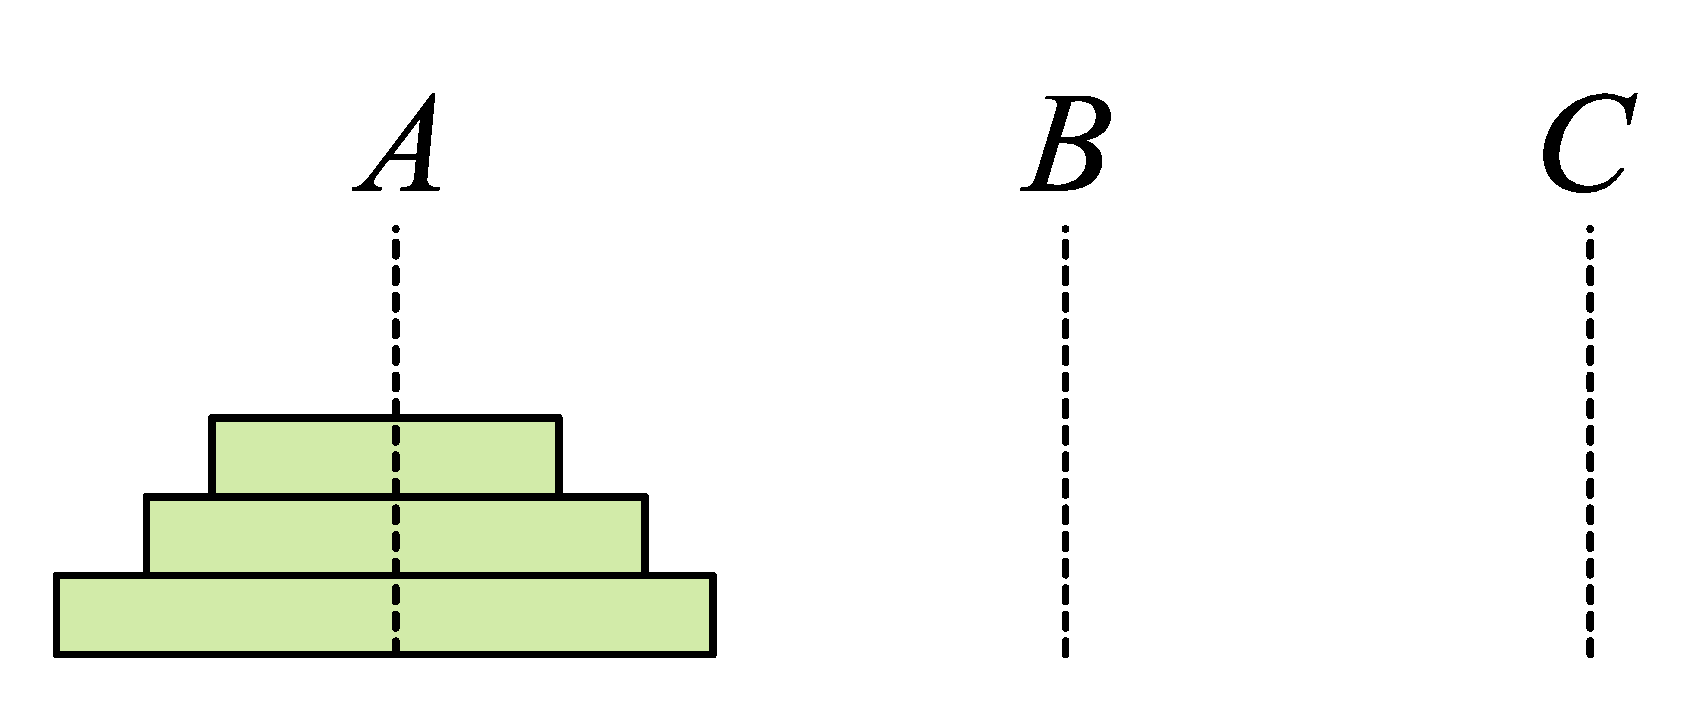
\includegraphics[width=0.35\textwidth]{images/title/汉诺塔问题.pdf}
		\caption{汉诺塔问题}
		\label{fig:汉诺塔问题}
	\end{figure}

	\solution
	\\

	该问题即为著名的汉诺塔问题, 递归式的求解算法描述为: 先将$A$上面的$n-1$个盘子移到$B$, 再将$A$中最下边的盘子移动到$C$, 再将$B$中的$n-1$个盘子移动到$C$上即可. 伪码描述为算法\ref{alg:汉诺塔算法}:
	\begin{algorithm}[H]
		\begin{algorithmic}[1]
		\Require{$n$个盘子从上往下、从小到大放在$A$柱}
		\Ensure{将$A$柱的圆盘移到$C$柱上}
		\If{$n$ == 1}
			\State move $(A, C)$;
		\Else
			\State $\textbf{Hanoi}(A, B, n-1)$;
			\State move $(A, C)$;
			\State $\textbf{Hanoi}(B, C, n-1)$;
		\EndIf
		\State \textbf{end \{Hanoi\}}
		\end{algorithmic}
		\caption{汉诺塔问题的递归算法$\textbf{Hanoi}(A, C, n)$}
		\label{alg:汉诺塔算法}
	\end{algorithm}
	易知$T(1)=1$, 根据上述伪码可知时间复杂度有递推方程
	\begin{align}
		T(n) = 2T(n-1)+1
	\end{align}
	于是通过递推得到
	\begin{align}
		T\left( n \right) &=2T\left( n-1 \right) +1=2\left( 2T\left( n-2 \right) +1 \right) +1 \notag
		\\
		&=2^2T\left( n-2 \right) +1+2^1 \notag
		\\
		&=2^3T\left( n-3 \right) +1+2^1+2^2 \notag
		\\
		&=2^{n-1}T\left( 1 \right) +1+2+\cdots +2^{n-2} \notag
		\\
		&=2^n-1 \notag
	\end{align}
	于是$T(n)=\Theta \left(2^n\right)$. 而且可以证明的是, 汉诺塔问题不存在多项式时间算法, 因此是一个难解的问题.
\end{homeworkProblem}

\pagebreak


\begin{homeworkProblem}

	给定含有$n$个不同数的数组$L=\left\{ x_1,x_2,\cdots, x_n \right\}$, 若$L$中存在$x_i$, 使得$x_1<x_2<\cdots<x_{i-1}<x_i>x_{i+1}>\cdots >x_n$, 则称$L$是单峰的, 并称$x_i$是$L$的峰顶. 假设$L$是单峰的, 设计一个优于$O(n)$的算法找到$L$的峰顶.
	\\

	\solution
	\\

	\textbf{算法思路描述:} 对区间$[0,n-1]$进行二分, 不妨设中点为mid$=\left\lfloor (n-1)/2\right\rfloor $. 
	
	观察中点的左右邻点: 
	\begin{itemize}
		\item \textbf{case1:} 若$L\left[ \mathrm{mid}-1 \right] <L\left[ \mathrm{mid} \right] <L\left[ \mathrm{mid}+1 \right]$, 则显然峰顶在右半区间$[\text{mid} +  1, n - 1]$, 在该区间继续二分搜索即可;
		\item \textbf{case2:} 若$L\left[ \mathrm{mid}-1 \right] >L\left[ \mathrm{mid} \right] >L\left[ \mathrm{mid}+1 \right]$, 则显然峰顶在左半区间$[0, \text{mid} -  1]$, 在该区间继续二分搜索即可;
		\item \textbf{case2:} 若$L\left[ \mathrm{mid}-1 \right] <L\left[ \mathrm{mid} \right] >L\left[ \mathrm{mid}+1 \right]$, 则显然峰顶就是$L\left[ \mathrm{mid} \right]$, 至此搜索完毕.
	\end{itemize}
	对应的算法伪代码见如下\footnote{具体的C++程序代码见下一页}:
	\begin{algorithm}[H]
		\begin{algorithmic}[1]
		\Require{$n$个不同数的数组$L[0,n-1]$且$L$为单峰数组}
		\Ensure{$L$的峰顶}
		\If{$n$ == 3} \Comment{因为已知$L$为单峰数组, 因此$n\geq 3$}
			\State \Return $L[1]$; \Comment{若$n=3$, 则显然$L[1]$为峰顶}
		\Else
			\State \textbf{int} low = 0, high = $n-1$;
			\While{low <= high}
				\State \textbf{int} mid = (low + high) $>>$ 1;
				\If{$L\left[ \mathrm{mid}-1 \right] <L\left[ \mathrm{mid} \right] >L\left[ \mathrm{mid}+1 \right]$}
					\State \Return $L\left[ \mathrm{mid} \right]$;
				\ElsIf{$L\left[ \mathrm{mid}-1 \right] <L\left[ \mathrm{mid} \right] <L\left[ \mathrm{mid}+1 \right]$}
					\State low = mid $+$ 1;
				\Else
					\State high = mid $-$ 1;
				\EndIf
			\EndWhile
		\EndIf
		\State \textbf{end \{peakIndex\}}
		\end{algorithmic}
		\caption{单峰数组的二分搜索算法$\textbf{peakIndex}(L)$}
		\label{alg:单峰数组的二分搜索算法}
	\end{algorithm}
	现在来分析算法的时间复杂度$T(n)$: 因为每一次二分都只需要做两次(常数次)比较, 所以$T(n)$的递归方程为$T\left( n \right) =T\left( n/2 \right) +O\left( 1 \right) $, 根据主定理($a=1,b=2,d=0$)可解得$T\left( n \right) =O\left( \log n \right) $.
	\newpage
	寻找单峰数组峰顶的C++程序(已在对应的\href{https://leetcode.cn/problems/B1IidL/}{\textbf{LeetCode题目}}上全部通过42个测试样例):
\begin{tcblisting}{listing engine=minted,boxrule=0.1mm,
colback=blue!5!white,colframe=blue!75!black,
listing only,left=5mm,enhanced,sharp corners=all,
overlay={\begin{tcbclipinterior}\fill[red!20!blue!20!white] (frame.south west)
rectangle ([xshift=5mm]frame.north west);\end{tcbclipinterior}},
minted language=c++,
minted style=tango,
minted options={fontsize=\small,breaklines,autogobble,linenos,numbersep=3mm}}
class Solution {
public:
    int peakIndexInMountainArray(vector<int>& arr) {
        int n = arr.size(), res = 0;
        if(n == 3) {
            res = 1;
        }
        else {
            int low = 1, high = n - 2;  //起始指针不要放两边, 否则会越界
            while(low <= high) {
                int mid = (low + high) >> 1;
                if(arr[mid - 1] < arr[mid]) {
                    low = mid + 1;
                }
                else if(arr[mid - 1] > arr[mid]) {
                    high = mid - 1;
                }
            }
            res = high;  //此时low > high, L[high]就是对应的峰顶
        }
        return res;
    }
};
\end{tcblisting}
\end{homeworkProblem}

\pagebreak

\begin{homeworkProblem}

	设$A$是$n$个不同元素组成且排好序的数组, 给定数$L$和$U$, $L<U$, 设计一个优于$O(n)$的算法, 找到$A$中满足$L<x<U$的所有数$x$.
	\\

	\solution
	\\

	\textbf{算法思路描述:} 我们需要分类讨论:
	\begin{itemize}
		\item 当$L>=A[n-1]$或$U<=A[0]$时, 显然数集$x=\emptyset$;
		\item 当$L<A[0]<U<A[n-1]$时, 用下述的\hyperref[alg:lowerbound算法]{\textbf{lowerbound算法}}找到数组$A$中第一个大于等于$U$的元素索引$q$, 则$x=\left\{ A\left[ 0 \right] ,A\left[ 1 \right] ,\cdots ,A\left[ q-1 \right] \right\}$; 
		\item 当$L=A[0]<U<A[n-1]$时, 则$x=\left\{ A\left[ 1 \right] ,A\left[ 2 \right] ,\cdots ,A\left[ q-1 \right] \right\}$;
		\item 当$A[0]<L<U<A[n-1]$时, 则先用\textbf{Problem 5}的\hyperref[alg:upperbound算法]{\textbf{upperbound算法}}找到数组$A$中第一个大于$L$的元素索引$p$, 再用\hyperref[alg:lowerbound算法]{\textbf{lowerbound算法}}找到数组$A$中第一个大于等于$U$的元素索引$q$, 这样就有$$x=\left\{ A\left[ p \right] ,A\left[ p+1 \right] ,\cdots ,A\left[ q-1 \right] \right\}$$
		\item 当$A\left[ 0 \right] <L<U=A\left[ n-1 \right] $时, 则用\hyperref[alg:upperbound算法]{\textbf{upperbound算法}}找到数组$A$中第一个大于$L$的元素索引$p$, 于是$x=\left\{ A\left[ p \right] ,A\left[ p+1 \right] ,\cdots ,A\left[ n-2 \right] \right\}$;
		\item 当$A\left[ 0 \right] <L<A\left[ n-1 \right] <U$时, 则用\hyperref[alg:upperbound算法]{\textbf{upperbound算法}}找到数组$A$中第一个大于$L$的元素索引$p$, 则$x=\left\{ A\left[ p \right] ,A\left[ p+1 \right] ,\cdots ,A\left[ n-1 \right] \right\}$;
	\end{itemize}
	  

	\begin{algorithm}[H]
		\begin{algorithmic}[1]
		\Require{长度为$n$的升序数组$A[0,\cdots,n - 1]$, 目标元素target}
		\Ensure{第一个大于等于target的元素下标}
		\State \textbf{int} low = 0, high = $n - 1$;
		\While{low $<=$ high}
			\State \textbf{int} mid = (low + high) $>>$ 1;
			\If{$A[\text{mid}] < \text{target}$}
				\State low = mid + 1;
			\Else
				\State high = mid $-$ 1;
			\EndIf
		\EndWhile
		\State \Return low; \Comment{返回所要求的下标}
		\State \textbf{end \{lowerbound\}}
		\end{algorithmic}
		\caption{二分查找\textbf{lowerbound}算法}
		\label{alg:lowerbound算法}
	\end{algorithm}
	此题主要在于分类讨论和第4种情况的求解, 其对应的C++程序非常简单(直接用一下STL的lower_bound和upper_bound二分查找函数即可), 故此处就不再罗列了. 而本文所构造的算法主要用到了两个二分查找的函数, 显然该算法的时间复杂度为$O(\log n)$, 是优于$O(n)$的.
\end{homeworkProblem}

\pagebreak

\begin{homeworkProblem}
	在$n$枚$(n\geq 3)$硬币中有一枚重量不合格的硬币(过轻或过重), 如果只有一架天平可以用来称重且称重的硬币数没有限制. 设计一个算法, 找出这枚不合格的硬币, 使得称重的次数最少(优于$O(n)$).
	
	(提示: 分成$n/3$或$n/4$份, 至少两份数量相等)
	\\

	\solution
	\\

	\textbf{算法思想描述:} 采用分治策略, 如果剩下的硬币个数小于3(即$n<3$), 则将其逐个与正常硬币(可以从拿走的硬币中随便选一个)相比较, 不等的那枚就是不合格的硬币; 若$n\geq 3$(即剩下的硬币个数至少是3), 则将这些硬币分成3份, 其中两份个数一样($k=\left\lfloor n/3\right\rfloor $), 另一份个数为$n-2k$. 将前两份称重对比, 若天平失衡则这两份中包含着异常硬币, 否则异常硬币在剩下的一份中. 递归进行划分处理, 直到$n<3$为止. 具体的算法伪代码见如下:
	\begin{algorithm}[H]
		\begin{algorithmic}[1]
		\Require{共$n$枚硬币(且含有1枚异常硬币)的集合$A$}
		\Ensure{1枚异常硬币}
		\State $k:=\left\lfloor n/3\right\rfloor $;
		\If{$n<3$}
			\State 将其逐个与正常硬币(从拿走的硬币中选一个)相比较并找到异常硬币; \Comment{递归终止条件}
		\Else
			\State 将集合$A$分成3份$X,Y,Z$, 其中$\left\lvert X\right\rvert =\left\lvert Y\right\rvert =k,\left\lvert Z\right\rvert =n-2k$;
			\If{$W(X)\neq W(Y)$} \Comment{$W(X),W(Y)$分别为$X,Y$的重量}
				\State $A:=X\cup Y$;
			\Else
				\State $A:=Z$;
			\EndIf
			\State $n:=\left\lvert A\right\rvert $;
			\State $\textbf{CoinDet}(A,n)$;
		\EndIf
		\State \textbf{end \{CoinDet\}}
		\end{algorithmic}
		\caption{硬币检验算法$\textbf{CoinDet}(A,n)$}
		\label{alg:CoinDet算法}
	\end{algorithm}
	根据上述伪代码我们可以写出最坏情形下的时间复杂度$T(n)$的递归方程\footnote{子问题的规模要么是$Z$的规模$n/3$(最好情形), 要么是$X\cup Y$的规模$2n/3$(最坏情形)}:
	\begin{align}
		T\left( n \right) =T\left( 2n/3 \right) +O\left( 1 \right) 
	\end{align}
	显然$a=1,b=3/2,d=0$, 故根据主定理可知$T(n)=O(\log n)$.

	最好情形下的时间复杂度$T(n)$的递归方程为
	\begin{align}
		T(n)=T(n/3)+O(1)
	\end{align}
	显然最好情形下$a=1,b=3,d=0$, 根据主定理可求得对应的时间复杂度也是$O(\log n)$.
	故不论最好最坏情形, 算法的时间复杂度都是$O(\log n)$, 显然优于$O(n)$.
	\newpage
\end{homeworkProblem}

\pagebreak

\begin{homeworkProblem}
	设$A=\left\{ a_1,a_2,\cdots ,a_n \right\} ,B=\left\{ b_1,b_2,\cdots ,b_m \right\}$是整数集合, 其中$m=O(\log n)$, 设计一个优于$O(nm)$的算法找出集合$C=A\cap B$.
	

	\solution

	\textbf{方法1 (基于哈希集合):} \textbf{算法思想描述:} 先用一个哈希集合存储数组$A$的元素\footnote{哈希集合中的元素查找的时间复杂度是$O(1)$, 且天然起到一个去重的作用}, 然后遍历数组$B$, 如果$B$中的元素在$A$对应的哈希集合中可以找到, 那么将该元素放进哈希集合res中, 最后将res转换为vector数组即可. 算法对应的C++代码如下(已在对应的\href{https://leetcode.cn/problems/intersection-of-two-arrays/}{\textbf{LeetCode T349}}上全部通过55个测试样例):
\begin{tcblisting}{listing engine=minted,boxrule=0.1mm,
colback=blue!5!white,colframe=blue!75!black,
listing only,left=5mm,enhanced,sharp corners=all,
overlay={\begin{tcbclipinterior}\fill[red!20!blue!20!white] (frame.south west)
rectangle ([xshift=5mm]frame.north west);\end{tcbclipinterior}},
minted language=c++,
minted style=tango,
minted options={fontsize=\small,breaklines,autogobble,linenos,numbersep=3mm}}
class Solution {
public:
    vector<int> intersection(vector<int>& nums1, vector<int>& nums2) {
        unordered_set<int> res;  //res为哈希集合是为了对结果进行去重
        unordered_set<int> nums(nums1.begin(), nums1.end());
        for(auto num : nums2) {
            if(nums.find(num) != nums.end()) {  //如果找到了,就放到res里
                res.insert(num);
            }
        }
        return vector<int>(res.begin(), res.end());  //将去重后得到的结果转为vector数组
    }
};
\end{tcblisting}
	现在来分析一下此方法的时空复杂度: 使用一个集合存储数组$A$中的元素需要$O(n)$的时间, 遍历集合$B$并判断元素是否在$A$的哈希集合中需要$O(m)$的时间, 因此总的时间复杂度为$O(m+n)=O(n)$. $A$的哈希集合所占用的空间为$O(n)$, 故空间复杂度为$O(n)$.

	\textbf{方法2 (排序+二分查找):} \textbf{算法思想描述:} 由于数组$B$比较短, 所以先对其进行排序, 然后遍历数组$A$的元素, 在排序后的$B$中使用二分查找来检索该元素, 若找到则放入$C$中. 算法伪码描述如下:
	\begin{algorithm}[H]
		\begin{algorithmic}[1]
		\Require{数组$A[0,\cdots,n-1],B[0,\cdots,m-1]$}
		\Ensure{数组$C$, 其中$C=A\cap B$}
		\State \textbf{vector<int>} $C$;
		\State $\textbf{sort}(B.\text{begin}(), B.\text{end}())$;  \Comment{对数组$B$进行原地排序}
		\For{$i=0$; $i<n$; $i$++}
			\State \textbf{bool} flag = $\textbf{binary_search}(B.\text{begin}(), B.\text{end}(), A[i])$;
			\If{flag == $\mathtt{true}$}
				\State $C.\textbf{push_back}(A[i])$;
			\EndIf
		\EndFor
		\State \Return $C$;
		\State \textbf{end \{Intersection\}} \Comment{算法的C++代码跟伪代码非常相似, 就不列出了}
		\end{algorithmic}
		\caption{数组交集算法\textbf{Intersection}}
		\label{alg:交集算法}
	\end{algorithm}
	现在来分析一下此方法的时空复杂度: 对$B$排序需要$O(m\log m)$的时间, 遍历+二分查找需要消耗$O(n\times \log m)$的时间, 所以总的时间复杂度为$O\left( m\log m \right) +O\left( n\log m \right) =O\left( \left( m+n \right) \log m \right) =O\left( n\log m \right) =O\left( n\log\log n \right)$; 而数组$B$排序所用到的栈空间为$O(\log m)$, 对$B$二分查找所需的栈空间为$O(\log m)$, 所以算法的空间复杂度为$O(\log m)=O(\log \log n)$.
	\newpage
\end{homeworkProblem}


\pagebreak

\begin{homeworkProblem}
	设$S$是$n$个不等的正整数的集合, $n$为偶数, 给出一个算法将$S$划分为子集$S_1$和$S_2$, 使得$\left\lvert S_1\right\rvert =\left\lvert S_2\right\rvert $且$\displaystyle \left| \sum_{x\in S_1}{x}-\sum_{x\in S_2}{x} \right|$达到最大, 即两个子集元素之和的差达到最大 (要求时间复杂度$T(n)=O(n)$).
	\\

	\solution
	\\
	
	\textbf{算法思想描述:} 先利用\textbf{PartSelect算法}选取数组$S$的第$n/2+1$小的元素, 并将该元素作为pivot并利用\textbf{Partition算法}来对数组$S$进行\textbf{一次划分}, 低区元素全部进入$S_2$, 高区元素和pivot都进入到$S_1$(由于$n$为偶数, 所以能够保证$\left| S_1 \right|=\left| S_2 \right|$), 这样就能够确保$\displaystyle \left| \sum_{x\in S_1}{x}-\sum_{x\in S_2}{x} \right|$达到最大. 
	算法伪码见如下:
	\begin{algorithm}[H]
		\begin{algorithmic}[1]
		\Require{数组$S[0,\cdots,n-1]$} \Comment{$n$为偶数, $S$的元素彼此互异都为正整数}
		\Ensure{$\displaystyle \max_{\left| S_1 \right|=\left| S_2 \right|} \left| \sum_{x\in S_1}{x}-\sum_{x\in S_2}{x} \right|$}
		\State \textbf{vector<int>} $S_1(n/2),S_2(n/2)$;
		\State \textbf{int} pivot = $\textbf{PartSelect}\left( S,0,n-1,n/2+1 \right)$; \Comment{求数组$S$第$n/2+1$小的元素, 可以认为是"中位数"}
		\State \textbf{int} low = 0, high = $n-1$; \Comment{对撞双指针做一次划分}
		\While{low < high}
			\While{low < high \&\& $S[\text{high}]$ >= pivot}
				\State high-\,-;
			\EndWhile
			\State $\textbf{swap}(S[\text{low}], S[\text{high}])$;
			\While{low < high \&\& $S[\text{low}]$ <= pivot}
				\State low++;
			\EndWhile
			\State $\textbf{swap}(S[\text{low}], S[\text{high}])$;
		\EndWhile
		\State \textbf{int} loc = low; \Comment{此时的loc即为pivot所处的最终下标}
		\State \textbf{copy}($S$.begin(), $S$.begin() + loc, $S_2$.begin()); \Comment{低区进入$S_2$}
		\State \textbf{copy}($S$.begin() + loc, $S$.begin() + $(n - \text{loc})$, $S_1$.begin()); \Comment{高区和pivot进入$S_1$}
		\State \Return $S_1,S_2$; \Comment{注意到$\text{loc}$其实就是$n/2$, 因此$n - \text{loc}$即为$n/2$}
		\State \Return $\textbf{accumulate}(S_1.\text{begin}(), S_1.\text{end}(), 0)-\textbf{accumulate}(S_2.\text{begin}(), S_2.\text{end}(), 0)$;
		\State \textbf{end \{MaxSubtract\}}
		\end{algorithmic}
		\caption{最大化子集和差算法\textbf{MaxSubtract}}
		\label{alg:最大化子集和差算法}
	\end{algorithm}

	现在来分析一下算法的时间复杂度: 调用\textbf{PartSelect算法}最坏需要$O(n)$的时间, \textbf{Partition算法}(核心是对撞双指针)需要$O(n)$的时间, 所以总的时间复杂度为$T(n)=O(n)+O(n)=O(n)$.
\end{homeworkProblem}



\pagebreak

\begin{homeworkProblem}
	考虑第三章PPT NO.17 $\textbf{Select}(A,k)$算法: 

	(1). 如果初始元素分组$r=3$, 算法的时间复杂度如何?
	(2). 如果初始元素分组$r=7$, 算法的时间复杂度如何?


	\solution
	

	\textbf{(1)}. 若$r=3$, 则3个元素一组的中间值$u$是该数组的第$2$小元素, 此数组至少有2个小于等于$u$; $\left\lfloor n/3\right\rfloor $个中间值中至少有$\left\lceil \left\lfloor n/3\right\rfloor /2\right\rceil $个小于等于这些中间值的中间值$v$. 因此, 数组$A$中至少有$2\ast \left\lceil \left\lfloor n/3\right\rfloor /2\right\rceil \geq \left\lfloor n/3\right\rfloor \geq n/3-1$个元素小于等于$v$. 即$A$中至多有$n-(n/3-1)=2n/3+1$个元素大于$v$. 同理, 至多有$2n/3+1$个元素小于$v$. 这样, 以$v$为划分元素所产生的新数组中至多有$2n/3+1$个元素. 既可以认为子问题的规模为$2n/3$. 求中位数的中位数所递归调用的规模为$n/3$, 一趟快排和插入排序的所需时间为$cn$. 综上, 时间复杂度的递推方程为
	\begin{align}
		T\left( n \right) =T\left( \frac{n}{3} \right) +T\left( \frac{2n}{3} \right) +cn
	\end{align}
	画出$T(n)$的递归树, 见如下图\ref{fig:递归树-1}:
	\begin{figure}[H]  % 这里记得用[H]
		\centering
		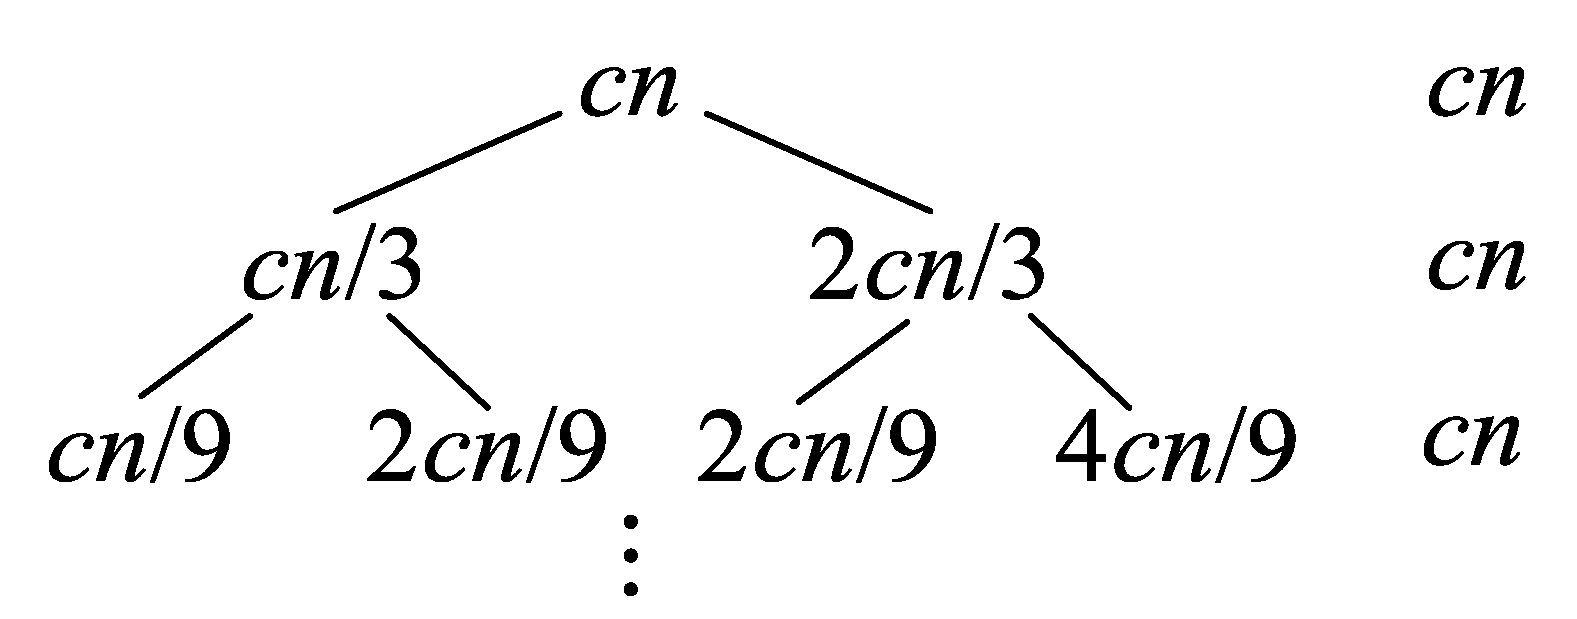
\includegraphics[width=0.4\linewidth]{images/title/递归树1.pdf}
		\caption{递归树-1}
		\label{fig:递归树-1}
	\end{figure}
	而递归树的深度为$\log n$, 而每一层的操作都是$cn$, 所以时间复杂度$T(n)=O(cn\log n)=O(n\log n)$;
	\textbf{(2)}.若$r=7$, 则7个元素一组的中间值$u$是该数组的第$4$小元素, 此数组至少有4个小于等于$u$; $\left\lfloor n/7\right\rfloor $个中间值中至少有$\left\lceil \left\lfloor n/7\right\rfloor /2\right\rceil $个小于等于这些中间值的中间值$v$. 因此, 数组$A$中至少有$4\ast \left\lceil \left\lfloor n/7\right\rfloor /2\right\rceil \geq 2\ast \left\lfloor n/7\right\rfloor \geq 2(n/7-1)$个元素小于等于$v$. 即$A$中至多有$n-2(n/7-1)=5n/7+2$个元素大于$v$. 同理, 至多有$5n/7+2$个元素小于$v$. 这样, 以$v$为划分元素所产生的新数组中至多有$5n/7+2$个元素. 既可以认为子问题的规模为$5n/7$. 求中位数的中位数所递归调用的规模为$n/7$, 一趟快排和插入排序的所需时间为$cn$. 综上, 时间复杂度的递推方程为
	\begin{align}
		T\left( n \right) =T\left( \frac{n}{7} \right) +T\left( \frac{5n}{7} \right) +cn
	\end{align}
	画出$T(n)$的递归树, 见如下图\ref{fig:递归树-2}:
	\begin{figure}[H]  % 这里记得用[H]
		\centering
		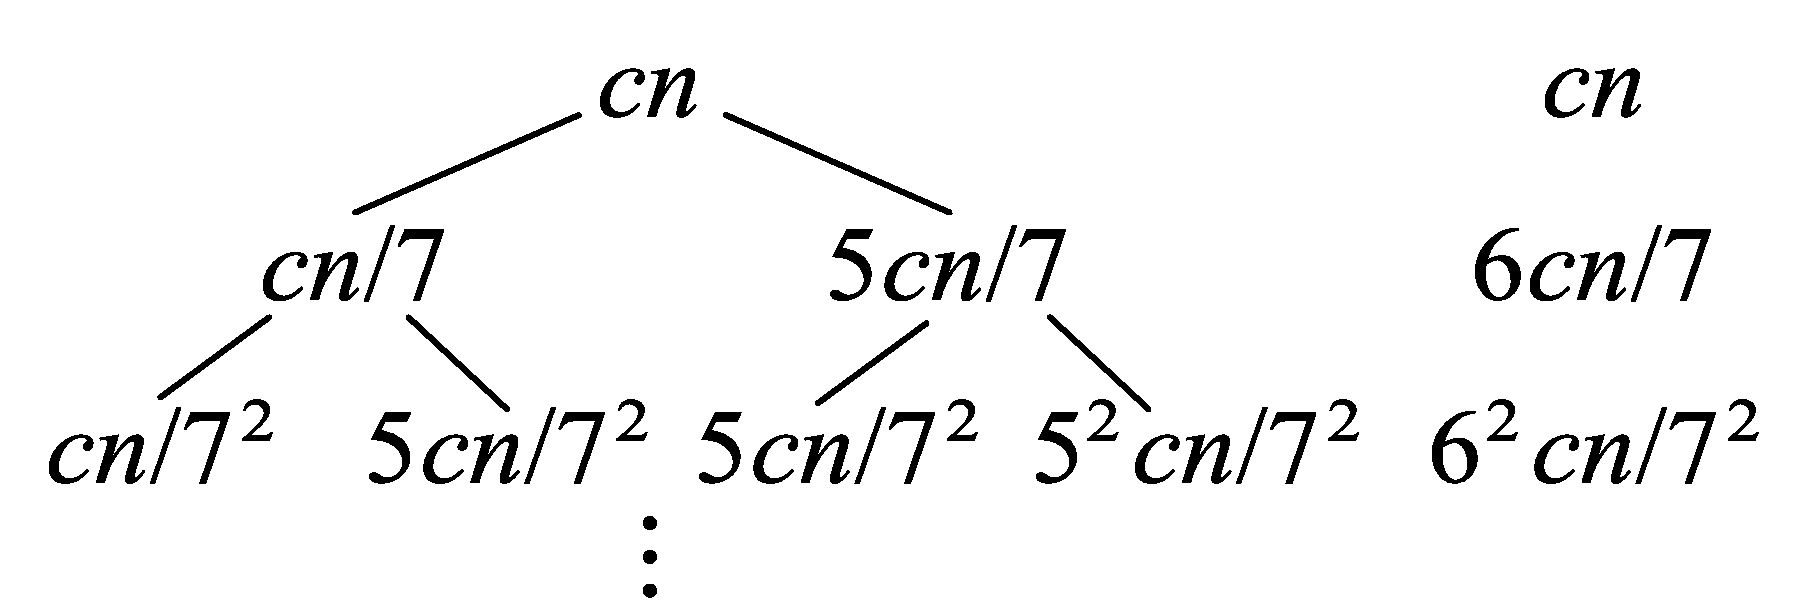
\includegraphics[width=0.4\linewidth]{images/title/递归树2.pdf}
		\caption{递归树-2}
		\label{fig:递归树-2}
	\end{figure}
	故总的时间复杂度为:
	\begin{align}
		T\left( n \right) =cn\left( 1+\frac{6}{7}+\left( \frac{6}{7} \right) ^2+\cdots \right) \le cn\cdot \frac{1}{1-\frac{6}{7}}=7cn=O\left( n \right) 
	\end{align}
\end{homeworkProblem}


\begin{homeworkProblem}
	在Internet上的搜索引擎经常需要对信息进行比较,比如可以通过某个人对一些事物的排名来估计他对各种不同信息的兴趣. 对于不同的排名结果可以用逆序来评价他们之间的差异. 考虑$1,2,\cdots,n$的排列$i_1,i_2,…,i_n$, 如果其中存在$i_j,i_k$, 使得$j<k$但$i_j>i_k$,那么就称$(i_j,i_k)$是这个排列的一个逆序. 一个排列含有逆序的个数称为这个排列的逆序数. 
	
	例如: 排列$(2 ,6 ,3 ,4 ,5 ,1)$含有8个逆序: (2,1),(6,3),(6,4),(6,5),(6,1),(3,1),(4,1),(5,1),它的逆序数就是8. 一个由$1,2,\cdots,n$组成的所有$n!$个排列中, 最小的逆序数是0, 对应的排列是$(1 ,2, 3, 4, \cdots, n)$,最大的逆序数是$n(n-1)/2$,对应的排列是$(n,n-1,\cdots,2,1)$. 逆序数越大的排列与原始排列的差异度越大. 利用二分归并排序算法设计一个计数给定排列逆序数的分治算法, 并对算法的时间复杂度进行分析.
	\\

	\solution
	\\
	
	\textbf{算法思想描述:} 在二分归并排序算法中\textbf{顺带做了}计数逆序的工作, 在递归调用算法分别对子数组$L_1,L_2$排序时, 分别计算每个子数组内部的逆序; 在归并排好序的子数组$L_1,L_2$的过程中, 计算$L_1$的元素与$L_2$的元素之间产生的逆序. 具体来说, 合并两个有序数组所采用的是双指针算法, 每当遇到当前左指针$i$所指元素$L_1[i]>$当前右指针$j$所指元素$L_2[j]$时, 意味着$L_1$中从指针$i$到末尾的所有元素都与$L_2[j]$构成逆序对, 于是此情形的逆序对增量为$\text{mid}-i+1$; 而当$L_1[i]<=L_2[j]$时, 则此情形对于逆序对增量的贡献为0(即没有逆序对). 算法伪代码见如下:
	\begin{algorithm}[H]
		\caption{双指针合并算法$\textbf{Merge}(\text{low, mid, high})$}
		\label{alg:合并过程}
		\begin{algorithmic}[1]
		\Require{排序后的子数组$A[\text{low}, \cdots, \text{mid}]$和$A[\text{mid}+1, \cdots, \text{high}]$} \Comment{双指针法合并两个有序数组}
		\Ensure{合并好的升序数组$A[\text{low}, \cdots, \text{high}]$及逆序数}
		\State \textbf{global} count = 0; \Comment{count是\textbf{int}型全局变量}
		\State \textbf{int} $k=0,\,i=\text{low},\,j=\text{mid}+1$; \Comment{$i,j$是拣取游标(即双指针), $k$是向$B$存放元素的游标}
		\State \textbf{vector<int>} $B$(high $-$ low + 1); \Comment{借用临时数组$B$}
		\While{$i\leq \text{mid}$ \&\& $j\leq \text{high}$} \Comment{当两个集合都没有取尽时}
		  \If{$A[i]\leq A[j]$}
			\State $B[k\text{++}]:=A[i\text{++}]$; \Comment{此情形对逆序数的增量是没有贡献的}
		  \Else
			\State $B[k\text{++}]:=A[j\text{++}]$;
			\State count += mid $-$ $i$ + 1; \Comment{此情形下, $L_1$中从指针$i$到末尾的所有元素都与$L_2[j]$构成逆序对}
		  \EndIf
		\EndWhile
		\While{$i\leq \text{mid}$} \Comment{当第二子组元素被取尽, 而第一组元素未被取尽时}
		  \State $B[k\text{++}]:=A[i\text{++}]$;
		\EndWhile
		\While{$j\leq \text{high}$} \Comment{当第一子组元素被取尽, 而第二组元素未被取尽时}
		  \State $B[k\text{++}]:=A[j\text{++}]$;
		\EndWhile
		\State \textbf{copy}($B$.begin(), $B$.end(), $A$.begin() + low) \Comment{将临时数组$B$中的元素拷贝给数组$A[\text{low},\cdots,\text{high}]$}
		\State \textbf{end\{Merge\}}
		\end{algorithmic}
	\end{algorithm}

	\begin{algorithm}[H]
		\caption{归并排序主程序伪码$\textbf{MergeSort}(\text{low, high})$}
		\label{alg:归并排序主程序伪码}
		\begin{algorithmic}[1]
		\Require{待排序的数组$A$及下标low,high}
		\Ensure{排序后的数组$A[\text{low},\cdots,\text{high}]$及$A$的逆序数} 
		\If{low < high}
		\State \textbf{int} $\text{mid} := \left\lfloor (\text{low}+\text{high})/2\right\rfloor $ \Comment{求当前数组的分割点}
		\State \textbf{MergeSort}(low, mid); \Comment{递归处理前半部分子数组}
		\State \textbf{MergeSort}(mid + 1, high); \Comment{递归处理后半部分子数组}
		\State \textbf{Merge}(low, mid, high); \Comment{归并两个排序后的子数组并计算逆序数}
		\EndIf
		\State \textbf{end\{MergeSort\}}
		\end{algorithmic}
	\end{algorithm}
	该算法对应的C++程序(已在对应的\href{https://leetcode.cn/problems/shu-zu-zhong-de-ni-xu-dui-lcof/}{\textbf{LeetCode题目}}上全部通过139个测试样例)为:
\begin{tcblisting}{listing engine=minted,boxrule=0.1mm,
colback=blue!5!white,colframe=blue!75!black,
listing only,left=5mm,enhanced,sharp corners=all,
overlay={\begin{tcbclipinterior}\fill[red!20!blue!20!white] (frame.south west)
rectangle ([xshift=5mm]frame.north west);\end{tcbclipinterior}},
minted language=c++,
minted style=tango,
minted options={fontsize=\small,breaklines,autogobble,linenos,numbersep=3mm}}
class Solution {
public:
    int count; //定义为全局变量
    int reversePairs(vector<int>& nums) {
        count = 0;
        MergeSort(nums, 0, nums.size() - 1);
        return count;
    }

    void Merge(vector<int>& nums, int low , int mid, int high) {
        int i = low, j = mid + 1, k = 0;
        vector<int> temp(high - low + 1);
        while(i <= mid && j <= high) {
            if(nums[i] <= nums[j])
                temp[k++] = nums[i++];  //此情形下逆序数没有增量
            else {
                temp[k++] = nums[j++];
                count += mid - i + 1;  //此情形下逆序数才能有增量
            }
        }
        while(i <= mid) temp[k++] = nums[i++];  //把剩下的nums左半数组接上
        while(j <= high) temp[k++] = nums[j++];  //把剩下的nums右半数组接上
        copy(temp.begin(), temp.end(), nums.begin() + low);  //把临时数组的元素拷贝回nums
        vector<int>().swap(temp);  //清除容器并最小化它的容量
    }
    
    void MergeSort(vector<int>& nums, int low, int high) {
        if(low < high) {
            int mid = (low + high) >> 1;
            MergeSort(nums, low, mid);
            MergeSort(nums, mid + 1, high);
            Merge(nums, low, mid, high);
        }
    }
};
\end{tcblisting}
显然该逆序数计算的算法伪码和C++代码跟归并排序算法几乎一模一样, 就比归并排序在第9行多了个count的加法运算, 但算法的关键操作还是比较. 所以此算法的时间复杂度递推公式跟归并排序一样:
\begin{align}
	T\left( n \right) =2T\left( n/2 \right) +O\left( n \right) 
\end{align}
易知$a=2,b=2,d=1$, 故根据主定理可知$T(n)=O(n\log n)$.
\end{homeworkProblem}

\begin{homeworkProblem}
	对玻璃瓶做强度试验, 设地面高度为0, 从0向上有$n$个高度, 记为$1,2,\cdots,n$, 其中任何两个高度之间的距离都相等. 如果一个玻璃瓶从高度$i$落到地上没有摔碎, 但从高度$i+1$落到地上摔碎了, 那么就将玻璃瓶的强度记为$i$.

	(1). 假设每种玻璃瓶只有1个测试样品, 设计算法来测试出每种玻璃瓶的强度. 以测试次数作为算法的时间复杂度, 估计算法的复杂度;

	(2). 假设每种玻璃瓶有足够多的相同的测试样品, 设计算法使用最少的测试次数来完成测试;

	(3). 假设每种玻璃瓶只有2个相同的测试样品, 设计次数尽可能少的算法完成测试.
	\\

	\solution
	\\

	\textbf{(1).} 顺序从下到上测试, 一次一个高度, 最坏情况下时间复杂度为$T(n)=O(n)$;

	\textbf{(2).} 因为高度越高, 玻璃瓶越容易碎, 其实可以理解为"升序数组". 因此我们可以考虑用二分法: 先在高度$n/2$测试玻璃瓶, 如果摔碎了, 则玻璃瓶的强度位于$[1,n/2-1)$(在该区间继续二分搜索即可); 若没摔碎, 则玻璃瓶的强度位于$[n/2+1,n]$(在该区间继续二分搜索即可). 显然, 该二分搜索的时间复杂度为$T(n)=O(\log n)$;
	
	\textbf{(3).} 不失一般性, 不妨设$\sqrt{n}$为整数, 则可以将$1,2,3,\cdots,n$这些$n$个高度分成$\sqrt{n}$组\footnote{如果$\sqrt{n}$不是整数, 则取$\left\lfloor \sqrt{n}\right\rfloor $个整组, 剩下的单独成一组}. 那么第$j$组($j=1,2,\cdots,\sqrt{n}$)所含有的高度有
	\begin{align}
		\left( j-1 \right) \sqrt{n}+1,\left( j-1 \right) \sqrt{n}+2,\cdots ,\left( j-1 \right) \sqrt{n}+\sqrt{n},\quad j=1,2,\cdots ,\sqrt{n}
	\end{align}

	先拿第一个瓶子测试: 从下往上, 按照每组的最大高度(即$j\sqrt{n},j=1,2,\cdots,\sqrt{n}$)进行测试. 如果前$j-1$组的测试中瓶子都没有碎, 而在第$j$组的测试中碎了, 则强度显然位于第$j$组的$\sqrt{n}$个高度中. 于是, 至多经过$\sqrt{n}$此测试, 待检查的高度范围就缩减到原来的$\frac{\sqrt{n}}{n}=\frac{1}{\sqrt{n}}$倍;

	再拿第二个瓶子测试: 在第$j$组的$\sqrt{n}$个高度中, 从下往上测试玻璃瓶的强度, 至多经过$\sqrt{n}$次测试, 就可以得到玻璃瓶的强度.

	现在来分析算法的时间复杂度: 显然第一个瓶子测验至多需要耗时$O(\sqrt{n})$, 第二个瓶子测试也至多需要耗时$O(\sqrt{n})$, 于是总的算法时间复杂度为
	\begin{align}
		T(n)=O(\sqrt{n})+O(\sqrt{n})=O(\sqrt{n})
	\end{align}
	\newpage
\end{homeworkProblem}

\pagebreak

\begin{homeworkProblem}
	\textbf{1.} 使用主定理求解以下递归方程:

	(1). $\begin{cases}
		T\left( n \right) =9T\left( n/3 \right) +n\\
		T\left( 1 \right) =1\\
	\end{cases}$;  (2). $\begin{cases}
		T\left( n \right) =5T\left( n/2 \right) +\left( n\log n \right) ^2\\
		T\left( 1 \right) =1\\
	\end{cases}$;  (3). $\begin{cases}
		T\left( n \right) =2T\left( n/2 \right) +n^2\log n\\
		T\left( 1 \right) =1\\
	\end{cases}$


	\solution
	

	\textbf{(1).} 易知$a=9,b=3,d=1,f(n)=n$, 由于$f\left( n \right) =n=O\left( n^{2-\epsilon} \right) $, 故根据主定理可知: 
	$T(n)=$
	
	$\Theta(n^2)$;

	\textbf{(2).} 易知$a=5,b=2,f(n)=n^2\log^2n=O(n^{\log_2 5-\epsilon})$, 故根据主定理可知$T(n)=\Theta \left( n^{\log_2 5} \right)$;

	\textbf{(3).} 易知$a=2,b=2,f(n)=n^2\log n=\Omega \left( n^{1+\epsilon} \right)$, 而且$$af\left( n/b \right) =2\left( n/2 \right) ^2\log \left( n/2 \right) =n^2/2\left( \log n-1 \right) \le 0.5n^2\log n\,\,\left( c=1/2<1 \right)$$
	故根据主定理可知$T(n)=\Theta(f(n))=\Theta(n^2\log n)$.

	\textbf{2.} 使用递归树求解: $\begin{cases}
		T\left( n \right) =T\left( n/2 \right) +T\left( n/4 \right) +cn\\
		T\left( 1 \right) =1\\
	\end{cases}$;
	
	\solution

	递归树见如下图\ref{fig:递归树-3}:
	\begin{figure}[H]  % 这里记得用[H]
		\centering
		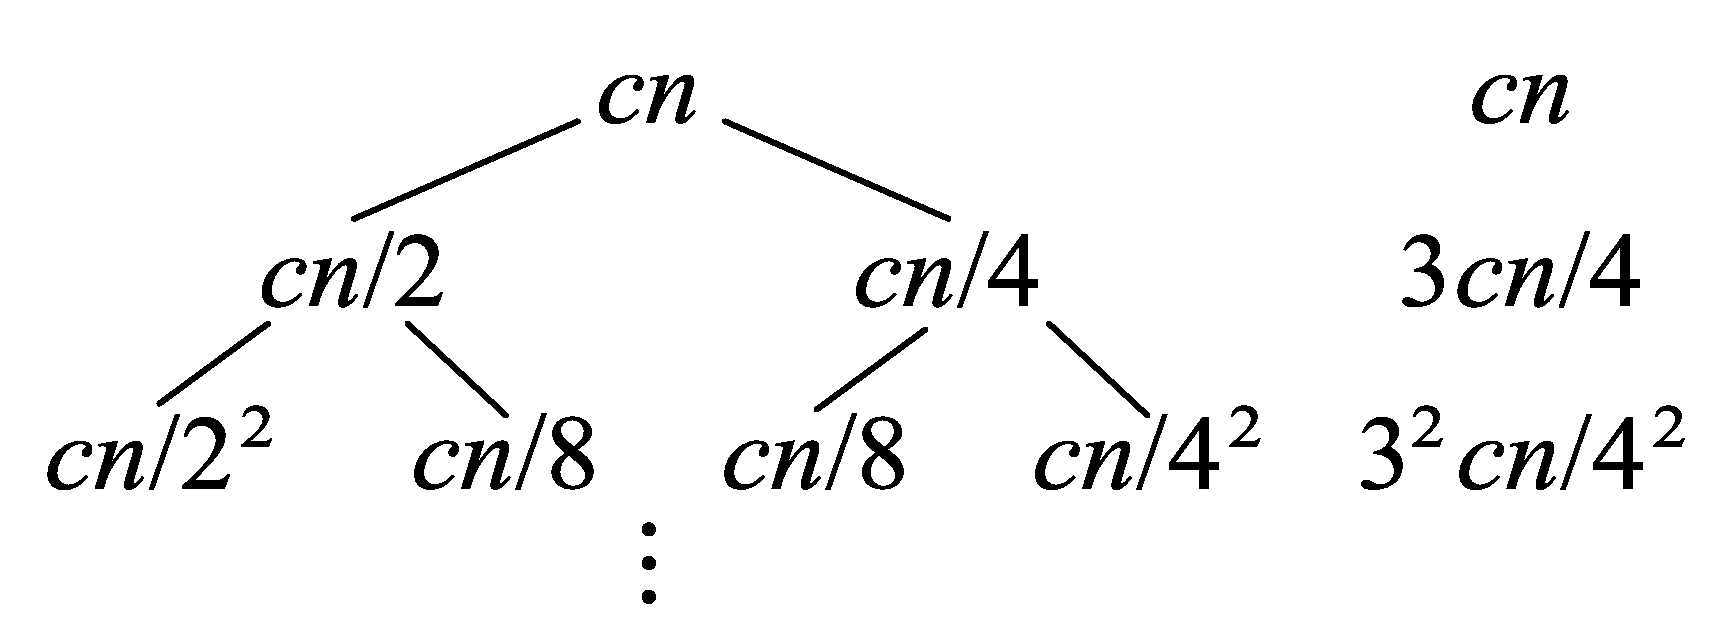
\includegraphics[width=0.4\linewidth]{images/title/递归树3.pdf}
		\caption{递归树}
		\label{fig:递归树-3}
	\end{figure}
	故总的时间复杂度为:
	\begin{align}
		T\left( n \right) =cn\left( 1+\frac{3}{4}+\left( \frac{3}{4} \right) ^2+\cdots \right) \le cn\cdot \frac{1}{1-\frac{3}{4}}=4cn=O\left( n \right) 
	\end{align}

	\textbf{3.} 使用迭代递归法求解: (1). $\begin{cases}
		T\left( n \right) =T\left( n-1 \right) +\log 3^n\\
		T\left( 1 \right) =1\\
	\end{cases}$;  (2). $\begin{cases}
		T\left( n \right) =T\left( n-1 \right) +1/n\\
		T\left( 1 \right) =1\\
	\end{cases}$.

	\solution

	\textbf{(1).} 易知
	\begin{align}
		T\left( n \right) &=T\left( n-1 \right) +\log 3^n=T\left( n-2 \right) +\log 3^{n-1}+\log 3^n
		\\
		&\cdots =T\left( 1 \right) +\log 3^2+\log 3^3+\cdots +\log 3^n
		\\
		&=1+\log \left( 3^{2+3+\cdots +n} \right) =1+\log \left( 3^{\left( n+2 \right) \left( n-1 \right) /2} \right) = \Theta \left(n^2\right)
	\end{align}

	\textbf{(2).} 易知
	\begin{align}
		T\left( n \right) &=T\left( n-1 \right) +\frac{1}{n}=T\left( n-2 \right) +\frac{1}{n-1}+\frac{1}{n}
		\\
		&\cdots =T\left( 1 \right) +\frac{1}{2}+\cdots +\frac{1}{n-1}+\frac{1}{n}=\sum_{i=1}^n{\frac{1}{i}}=\Theta \left( \gamma +\log n \right) =\Theta \left( \log n \right) 
	\end{align}
	注意, 其中我们用到了$\gamma$常数的数学结论: $\displaystyle \gamma = \lim_{n\to +\infty}\left(\sum_{i=1}^{n}\frac{1}{i}-\ln n\right)$.
\end{homeworkProblem}


% 引用文献
\bibliographystyle{unsrt}  % unsrt:根据引用顺序编号
\bibliography{refs}


\end{document}
